
\section{Geometric and electrical modeling \DDC}
\label{chap4:sect:geomModel}
%\input{4_thinning/figures/geomSubCurr}
To begin with, we will address the geometric approach.
It has been chosen thanks to the advantages it brings forward, such as the abstraction from electronics it enables, thus allowing easier and faster modeling.
However, because this approach alone is insufficient, we will then study an analogous electrical one.

\subsection{Geometric modeling \DDC}
\label{chap4:sect:geomModel:subsect:geomModel}
%\begin{figure}[!h]
%    \centering
%    \includegraphics[width=16cm]{4_thinning/figures/geomCrossView.pdf}
%    \caption{BBI susceptibility area cross-sectional view}
%    \label{fig:geomCrossView}
%\end{figure}

\begin{figure}[!h]
    \centering
    \begin{subfigure}{16cm}
        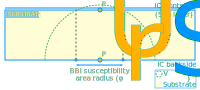
\includegraphics[width=16cm]{4_thinning/figures/geomCrossViewNew.pdf}
        \caption{Normal IC}
        \label{fig:geomCrossView;subfig:geomThick}
    \end{subfigure}
    \begin{subfigure}{16cm}
        \includegraphics[width=16cm]{4_thinning/figures/geomCrossViewThinNew.pdf}
        \caption{Thinned IC}
        \label{fig:geomCrossView;subfig:geomThin}
    \end{subfigure}
    \caption{BBI susceptibility area cross-sectional 2D view}
    \label{fig:geomCrossView}
\end{figure}
For the purpose of geometric modeling, let us consider two identical ICs.
A commercial one, with an arbitrary standard substrate thickness, and another one with its substrate thinned by a certain amount in order to perform fault injection.
Fig. \ref{fig:geomCrossView} illustrates the two-dimensional cross-sectional views of the considered ICs substrates during an arbitrary BBI voltage pulse.
The silicon substrate being an isotropic resistive environment, it is quite natural to expect the electrical charges to flow and spread evenly when injected into it at any given time.
Therefore, equipotentials form half-sphere surfaces inside the substrate volume.
These surfaces are highlighted in two-dimensions as green half-circles in Fig. \ref{fig:geomCrossView}.

In this scenario, an attacker wants to induce a fault in the logic gates, located at the top of each IC.
To that end, they need to change the voltage enough at point $P$, called $V_P$, in order to disturb the transistors and change the logic gates behavior.
In addition to that, and for the sake of simplicity, let us assume that $P$ is the only location in the considered IC where faults can be injected.
However, in order to observe faults at point $P$, $V_P$ needs to reach a minimal threshold voltage, called $V_F$.
Because the attacker is working with BBI, a metallic probe is connected onto the backside of the IC, at point $P_U$, in order to inject energy into the IC.
Depending on the amount of injected energy, in other words, the maximum amplitude of the voltage pulse because the substrate effective resistance is static, the voltage at $P$ might never reach $V_F$, therefore, no faults will be observed.
Let us consider that the attacker chose an amplitude $V_{PU}$ big enough such that at a moment in the injection, $V_P$ reaches $V_F$ or more in each considered IC.
In that scenario, the area on the IC front side where $V > V_F$ is a disk of radius $\phi$, centered in $P$, called the BBI susceptibility area radius.
It means that the attacker can position the probe anywhere on the backside within this disk to reach $V_F$ at $P$, and therefore induce a fault at $P$.

The half-sphere equipotential radius relative to time can be determined thanks to the following formula:
\begin{equation}
    r(t) = \frac{\rho_{SUB}}{\sqrt{2}} \cdot \frac{|I_G(t)|}{|V_{PU}(t) + V_F|}
\end{equation}
with $\rho_{SUB}$ the resistivity of the silicon substrate, $I_G(t)$ the instantaneous sum of the current distribution contained in the half-sphere, and $V_{PU}(t)$ the instantaneous voltage pulse applied on the backside of the IC.
Then, logically, the BBI susceptibility area radius, denoted $\phi_r$, is described by:
\begin{equation}
    \phi_r(t) = 2 \cdot \sqrt{r(t)^2 - t^2_{SUB}}
\end{equation}
with $t_{SUB}$ being the IC substrate thickness.

As it is illustrated in Fig. \ref{fig:geomCrossView}, thinning the substrate inevitably increases the size of the susceptibility area if the experimental conditions are constant.
It means that the susceptibility evolution ratio is always greater than 1 when thinning the substrate:
\begin{equation}
    \frac{\phi_r^{THIN}}{\phi_r^{THICK}} = \sqrt{\frac{r^2 - t^2_{THIN}}{r^2 - t^2_{THICK}}} > 1
\end{equation}

Therefore, in order to obtain the same susceptibility area with a thinner IC, it is required to reduce the voltage pulse amplitude, thanks to the following relation:
\begin{equation}
    \label{chap4:sect:geomModel:eqnVpu*}
    V_{PU}^* = \frac{t_{THIN}}{t_{THICK}} \cdot V_{PU} + V_F \cdot (1 - \frac{t_{THIN}}{t_{THICK}})
\end{equation}

Eventually, this geometrical approach allows deducing three conclusions:
\begin{enumerate}
    \item Thinning the substrate allows reducing the minimal voltage pulse amplitude required to induce a fault while keeping a constant susceptibility area.
    \item The BBI susceptibility area increases while the substrate thickness decreases while working at a constant voltage pulse $V_{PU}$.
    \item Thinning the substrate alone does not have an influence on BBI spatial resolution, as the susceptibility area depends on the couple $(t_{SUB}, V_{PU})$. Thus, similar spatial resolution could be obtained with different substrate thicknesses by changing $V_{PU}$.
\end{enumerate}

\newpage
\subsection{Electrical approach \DDC}
\label{chap4:sect:geomModel:subsect:elecApproach}
%\begin{figure}[H]
%    \centering
%    
\includegraphics[width=16cm]{4_thinning/figures/simuSubCoupe.pdf}
%    \caption{Non-thinned (140 µm) simulated IC substrate cross-sectional view}
%    \label{fig:simuSubCoupe}
%\end{figure}

%    trim={left lower right upper}
% THICK IC
\begin{figure}[H]
    \centering
    \begin{subfigure}{17cm}
        \centering
        \includegraphics[width=17cm, trim={3cm 2cm 0 3cm}, clip]{4_thinning/figures/simuSubCoupeVoltageTripleWellApex140um.pdf}
        \caption{Cross-sectional view (Y-axis)}
        \label{fig:simuSubCoupeThick;subfig:yaxis}
    \end{subfigure}
    \begin{subfigure}{16cm}
        \centering
        \includegraphics[width=16cm, trim={1cm 3cm 0.5cm 3.5cm}, clip]{4_thinning/figures/simuSubBottomVoltageTripleWellApex140um.pdf}
        \caption{Probe point of view}
        \label{fig:simuSubCoupeThick;subfig:bottom}
    \end{subfigure}
    \caption{Simulated non-thinned IC (140 µm) substrate voltage distribution: peak of the first voltage pulse edge}
    \label{fig:simuSubCoupeThick}
\end{figure}

% THIN IC
\begin{figure}[H]
    \centering
    \begin{subfigure}{17cm}
        \centering
        \includegraphics[width=17cm, trim={3cm 4.8cm 0 5.5cm}, clip]{4_thinning/figures/simuSubCoupeVoltageTripleWellApex60um.pdf}
        \caption{Cross-sectional view (Y-axis)}
        \label{fig:simuSubCoupeThin;subfig:yaxis}
    \end{subfigure}
    \begin{subfigure}{16cm}
        \centering
        \includegraphics[width=16cm, trim={1cm 3cm 0.5cm 3.5cm}, clip]{4_thinning/figures/simuSubBottomVoltageTripleWellApex60um.pdf}
        \caption{Probe point of view}
        \label{fig:simuSubCoupeThin;subfig:bottom}
    \end{subfigure}
    \caption{Simulated thinned IC (60 µm) substrate voltage distribution: peak of the first voltage pulse edge}
    \label{fig:simuSubCoupeThin}
\end{figure}

As stated previously, in order to verify the meaningfulness of the geometrical approach, we will complete it with an electrical modeling approach.
For this purpose, the models introduced in Chapter \ref{chap:3icModeling} are reused.
The electrical approach consists in generating ICs with different substrate thicknesses and simulating them during BBI.
The considered ICs are 550 µm wide and 450 µm deep.
%It consists in utilizing the models presented in Chapter \ref{chap:3icModeling} with different substrate thicknesses.
%To that end, the same IC will be used, with an 550 µm width and an 450 µm depth.
Two substrate thicknesses are analyzed, 60 µm and 140 µm.
The simulation parameters are the following:
\begin{itemize}
    \item Triple-well substrate
    \item Required voltage pulse: -300 V
    \item Required pulse width: 20 ns
    \item Required rise and fall times: 8 ns
\end{itemize}

Fig. \ref{fig:simuSubCoupeThick} and Fig. \ref{fig:simuSubCoupeThin} show, for each simulated IC, the voltage bias across the substrate through different point of view at the apex of the voltage pulse first edge.
For the sake of simplicity, results are shown in two dimensions and from two point of views.
A cross-sectional view and a bottom view are displayed.
The first interesting thing to note is that, as predicted thanks to the geometric model and as shown in Fig. \ref{fig:simuSubCoupeThick} and \ref{fig:simuSubCoupeThin}, equipotentials effectively form half-circles (half-spheres in 3D).
They can be observed thanks to both point of views.
\textcolor{orange}{IL Y A BEAUCOUP DE CHOSES À DIRE MAIS JE MANQUE D'INSPIRATION POUR CETTE PARTIE, JE REVIENDRAI PLUS TARD DESSUS.}
